
\begin{center}
\Huge
Ligningen for en tangent.
\end{center}
\section*{Hvordan vi finder ligningen for tangenten i et punkt}
\stepcounter{section}
Vi husker på, at hældingen af tangenten i et punkt $(x_0,f(x_0))$ for en differentiabel funktion $f$ er givet ved $f'(x_0)$. Ligningen for en ret linje er givet som 
\begin{align*}
y = ax+b,
\end{align*}
så ligningen for tangenten for $f$ i punktet $(x_0,f(x_0))$ må have $a = f'(x_0)$. 

En ret linje er entydigt bestemt ved hældningen og et punkt. Vi ved, at tangenten går gennem punktet $(x_0,f(x_0))$, så vi kan finde $b$ i ligningen ved at indsætte dette punkt i ligningen $y = f'(x_0)x+b$:
\begin{align*}
f(x_0) = f'(x_0)x_0+b &\Leftrightarrow b = f(x_0)-f'(x_0)x_0,
\end{align*}
og vi har løst $a$ og $b$ og dermed tangentens ligning.
\begin{exa}
Vi ønsker at finde ligningen for tangenten til funktionen $x^2$ i punktet $(1,1)$. Vi finder først den afledede til $x^2$:
\begin{align*}
(x^2)' = 2x.
\end{align*}
Derfor må hældningen af tangenten i punktet $(1,1)$ være $a = f'(1) = 2$. Vi skal nu finde $b$ i ligningen $y=2x+b$, så vi indsætter vores kendte punkt:
\begin{align*}
y = 2x+b \Leftrightarrow 1= 2\cdot 1 +b \Leftrightarrow b = -1,
\end{align*}
og derfor må tangentens ligning i punktet $(1,1)$ være givet som
\begin{align*}
y = 2x-1.
\end{align*}
Funktionen $x^2$ og tangenten i punktet $(1,1)$ til $x^2$ fremgår af Fig. \ref{fig:tangent}.
\begin{figure}[H]
\centering
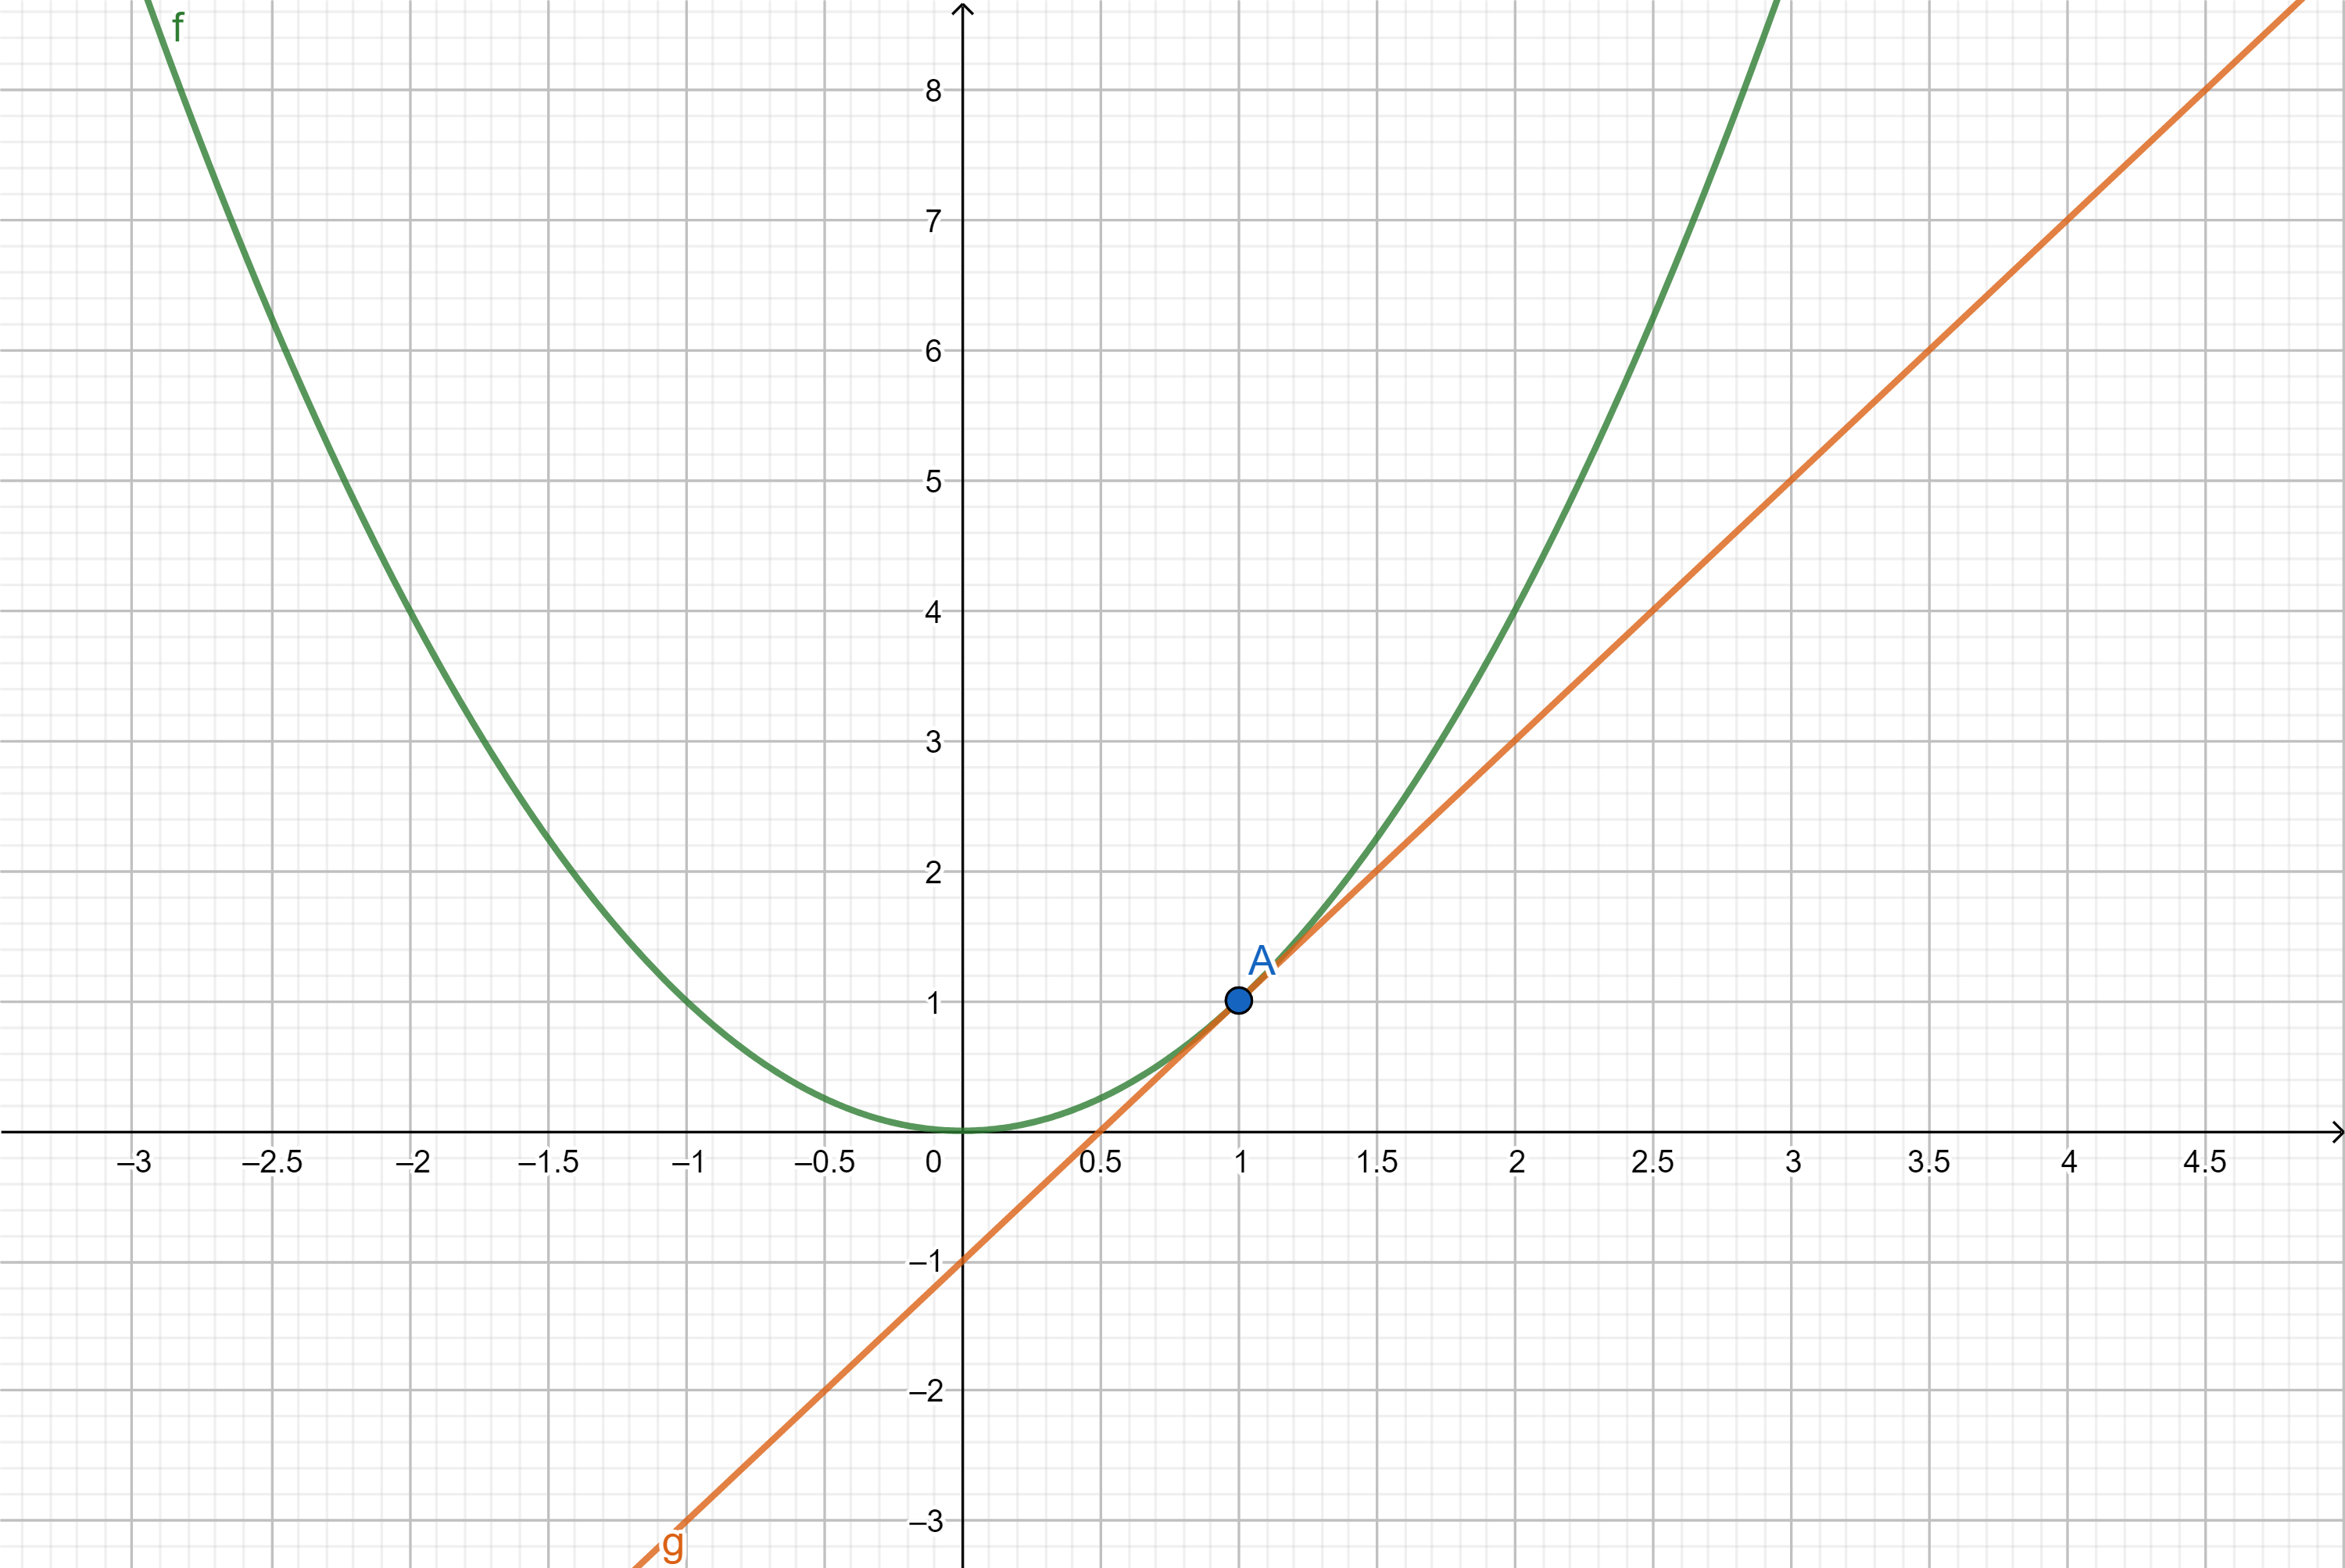
\includegraphics[scale=0.9]{Billeder/tangenthaeld.png}
\caption{Funktion $f(x)=x^2$ og tangentlinjen $g(x) = 2x-1$.}
\label{fig:tangent}
\end{figure} 
\end{exa}
Vi kan også bruge differentialregning til at sige noget om, hvad tallet $b$ betyder i et andengradspolynomium
\begin{align*}
f(x) = ax^2+bx+c.
\end{align*}
Vi ved allerede, at $c$ er $y$-værdien for skæringen med $y$-aksen. Desuden ved vi, at fortegnet på $a$ afgør, om vores parabel for andengradspolynomiet er "sur" eller "glad" - peger armene ned eller op. Differentierer vi $f$ får vi
\begin{align*}
f'(x) = 2ax+b,
\end{align*}
og indsætter vi så $x = 0$, får vi, at $f'(0) = b$. $b$ må derfor tilsvare hældningen af $f$ i punktet $(0,f(0))$, altså der, hvor grafen for $f$ skærer $y$-aksen. Desuden ved vi, at $f(0) = c$. Vi kan samle disse betragtninger til en sætning:
\begin{setn}
Ligningen for tangenten til funktionen $f(x) = ax^2+bx+c$ i punktet $(0,c)$ er givet ved
\begin{align*}
y = bx+c.
\end{align*}
\end{setn}

\section*{Bevis for differentialkvotienten af $x^2$}
\stepcounter{section}
\begin{setn}
Funktionen $f(x)=x^2$ er overalt differentiabel med differentialkvotient
\begin{align*}
\frac{d}{dx}x^2 = (x^2)' = 2x. 
\end{align*}
\end{setn}
\begin{proof}
Vi anvender definitionen af differentialkvotienten:
\begin{align*}
f'(x) = \lim_{h\to 0}\frac{f(x+h)-f(x)}{h},
\end{align*}
hvilket i tilfældet $f(x) = x^2$ giver
\begin{align*}
(x^2)' &= \lim_{h\to 0}\frac{(x+h)^2-x^2}{h}\\
&= \lim_{h\to 0} \frac{x^2+h^2+2xh-x^2}{h}\\
&= \lim_{h\to 0} \frac{h^2+2xh}{h}\\
&= \lim_{h\to 0} \frac{h^2}{h} + \lim_{h\to 0} \frac{2xh}{h}\\
&= \lim_{h\to 0} h + \lim_{h\to 0} 2x\\
&= 2x.
\end{align*}
\end{proof}

\section*{Opgave 1}
Find ligningen for tangenten til følgende funktioner i de tilhørende punkter:
\begin{align*}
&1) \ f(x) = x^2,\  p=(-1,f(-1))  &&2) \   f(x)=2x^2-1x+3, \ p=(0,f(0))    \\
&3) \ f(x) = \frac{1}{x} -x^3, \ p=(2,f(2))   &&4) \ f(x) = \sqrt{x}, \ p=(4,f(4))    \\
&5) \ f(x) = 7x+3,\ p=(3,f(3))   &&6) \ f(x) = -3x^2+5x-1, \ p=(1,f(1))     \\
&7) \ f(x) = 27, \ p= (1000,f(1000))   &&8) \ f(x) = 3x^2-2\sqrt{x}, \ p=(9,f(9))     \\
&9) \ f(x) = \frac{10}{x}+3x^3, \ p= (2,f(2))   &&10) \ f(x) = 5x^3+2x^2+x+1, \ p=(-2,f(-2))     \\
\end{align*}

\section*{Opgave 2}
Skitsér følgende polynomier:
\begin{align*}
&1) \ 2x^2+2x+3     &&2) \ -x^2 +10   \\
&3) \  3x^2-2x-4    &&4) \ -2x^2-3x-3  \\
\end{align*}